%%
%% This is file `sample-sigconf.tex',
%% generated with the docstrip utility.
%%
%% The original source files were:
%%
%% samples.dtx  (with options: `sigconf')
%% 
%% IMPORTANT NOTICE:
%% 
%% For the copyright see the source file.
%% 
%% Any modified versions of this file must be renamed
%% with new filenames distinct from sample-sigconf.tex.
%% 
%% For distribution of the original source see the terms
%% for copying and modification in the file samples.dtx.
%% 
%% This generated file may be distributed as long as the
%% original source files, as listed above, are part of the
%% same distribution. (The sources need not necessarily be
%% in the same archive or directory.)
%%
%% The first command in your LaTeX source must be the \documentclass command.
\documentclass[sigconf]{acmart}
\usepackage{indentfirst}
%%%% As of March 2017, [siggraph] is no longer used. Please use sigconf (above) for SIGGRAPH conferences.

%%%% Proceedings format for SIGPLAN conferences 
% \documentclass[sigplan, anonymous, review]{acmart}

%%%% Proceedings format for SIGCHI conferences
% \documentclass[sigchi, review]{acmart}

%%%% To use the SIGCHI extended abstract template, please visit
% https://www.overleaf.com/read/zzzfqvkmrfzn

%%
%% end of the preamble, start of the body of the document source.
\begin{document}

\title{RNA\_LZW: A Novel Method for Detection of Stems and Pseudoknotted Structures in Non-Coding RNA}

\author{Claire Champernowne}
\email{cchampernowne@gmail.com}
\affiliation{%
  \institution{University of Victoria}
}

\author{Quinn Gieseke}
\email{qgieseke@gmail.com}
\affiliation{%
  \institution{University of Victoria}
}

\renewcommand{\shortauthors}{Champernowne and Gieseke, et al.}

\begin{abstract}
  A clear and well-documented \LaTeX\ document is presented as an
  article formatted for publication by ACM in a conference proceedings
  or journal publication. Based on the ``acmart'' document class, this
  article presents and explains many of the common variations, as well
  as many of the formatting elements an author may use in the
  preparation of the documentation of their work.
\end{abstract}

%%
%% Keywords. The author(s) should pick words that accurately describe
%% the work being presented. Separate the keywords with commas.
\keywords{pseudoknot, non-coding RNA, secondary structure, tertiary structure, dot-bracket notation}

\maketitle




\section{Introduction}
Detecting RNA secondary structures is a process which is integral to understanding the functions of non-coding RNA sequences. Though there are existing bioinformatics tools used for detection, these programs are not without their limitations. 

Specifically, RNAz uses a sliding window approach in its analysis of a sequence \cite{RNAZ2} \cite{Fast}, meaning there may be structures with loops existing outside the scope of the window.

Additionally, it has been proven that utilizing current mimimum free energy calculations for the purposes of predicting pseudoknotted structures is NP-Complete \cite{NP}

The Lempel-Ziv-Welch (LZW) algorithm is a universal lossless compression algorithm used for a variety of applications such as Unix file compression. The algorithm compresses data by using a dictionary to assign common sequences of characters to a fixed-length code (typically 12-bit) \cite{compres}.

Because RNA structure exists in a 3-dimensional capacity, with its final form assuming a tertiary structure, base pairings which may appear to be distant from one another in a secondary structure can in reality exist very closely to one another once their tertiary structure is assumed. Given the LZW algorithm’s dictionary approach to pattern-matching,  RNA\_LZW can detect the presence of distant pseudoknots in a structure in much the same way that it detects regular base pairing. 

We propose that RNA\_LZW could serve as a pre-processing step to determine if there are notable base pairings throughout a given sequence, which may not be accounted for by standard secondary structure detection methods.

\section{algorithms}


\subsection{Lempel-Ziv-Welch Encoding}

RNA\_LZW uses only the encoding step of the LZW compression algorithm.  A high level overview of the encoding portion of the LZW algorithm as employed in RNA\_LZW is shown below:

\begin{enumerate}
\item Initialize the dictionary to contain all keys of length one. 
	\begin{enumerate}
		\item In this case, the dictionary initially contains only four characters; A,U,C, and G. 
	\end{enumerate}
\item Initialize a buffer as the first character in the sequence.
\item Add characters from the sequence to the buffer until the buffer represents a key that is not already represented in the dictionary. Once the buffer is added to the dictionary as a key, it is reset to just the last character.
	\begin{enumerate}
		\item Though not represented in a normal LZW algorithm, RNZ\_LZW records additional metadata about the position of the buffer in the greater sequence into the dictionary.
	\end{enumerate}
\item Though LZW encoding normally cannot iterate multiple times due to its need to be decoded without the dictionary; RNA\_LZW acts with global information, and does not have that restriction, and therefore uses multiple iterations to build a much more robust dictionary.
\end{enumerate}


\subsection{Dot-Bracket Construction}
Once we have the dictionary with many possible base matches, we must remove overlapping matches, and place only the most likely ones into the final output. Currently we measure stem likelihood first by length, and then by distance. The steps are as follows:
\begin{enumerate}
\item Remove impossible matches.
	\begin{enumerate}
	\item While adding entries to the dictionary, it is possible to add overlapping matches, where a sequence of bases can be paired with itself. For example, the sequence \texttt{UGAUAGCA} when reversed will exactly pair to itself. 
	\end{enumerate}
\item For each dictionary entry, parse the possible match locations and select the pair of base sequences that are the shortest distance apart.
\item Sort by match length.
\item Check the location of each stem placement in the output:
	\begin{enumerate}
	\item If the location is empty, add the stem to the output, marked by a unique key at every base location along the stem
	\item If any base in the location already has a stem, skip. Since we iterate from longest stems down to shortest, this biases the algorithm towards including longer stems.
	\end{enumerate}
\end{enumerate}


At this point in the algorithm, the output consists of a unique symbol per stem (The index in the output of the start of the right stem half), that is replicated at each base in the stem. To convert into standard dot-bracket notation, we must essentially reduce the number of bracket symbols down. For the purposes of notating pseudoknots, we use the bracket progression of \verb|{([{<ABCD| for opening brackets, and \verb|dcba>}])| for closing braces.

This algorithm utilizes a single modified stack in order to match braces as it progresses through the output sequence. The stack is allowed to have "transparent" entries that stay on the stack, but peek and pop operations will return the first non-transparent entry on the stack.
\begin{enumerate}
	\item Iterate through the output, left to right.
		\begin{enumerate}
		\item If the current value equals the top of the stack, pop the top of the stack. This is equivalent to finding a normal brace match
		\item If the current value equals the index of the match, and that value is not on top of the stack, then we have a closing bracket with its requisite opening bracket must be beyond the last opening bracket, meaning we have found a pseudoknonot.
			\begin{itemize}
			\item Since representing a pseudoknot requires a new style of brace, we iterate through the stack between the opening and closing brace (including transparent entries), seeking out the highest value of brace. We then assign a one higher value of brace to the current pair, and make both entries transparent. 
			\end{itemize}
		\item If neither of the above cases are true, we have a normal opening brace. Push current value to the stack.
		\end{enumerate}
\end{enumerate}

Finally, we iterate through the output one more time, converting each unique id into its corresponding brace value, and replacing any gaps with the '.' character.


\section{results}

In order to test for RNA\_LZW's efficacy as a preprocessing(?) step in identifying potentially relevant stems and pseudoknots in a given structure, it was tested using sequences where the secondary structure is known.  All sequences used were sourced from the RNACentral database. The dot-bracket notations of these known sequences were then compared to the dot-bracket output generated by RNA\_LZW both visually and using a \% similarity string comparison. It should also be noted that RNA\_LZW does not, in its current state, take wobble base pairing into account and is therefore incapable of finding the exact base pairings that occur in the known dot-bracket structures. 


\subsection{Homo sapiens tRNA-SeC (anticodon TCA) 1-1 (TRU-TCA1-1)}

\begin{figure}
  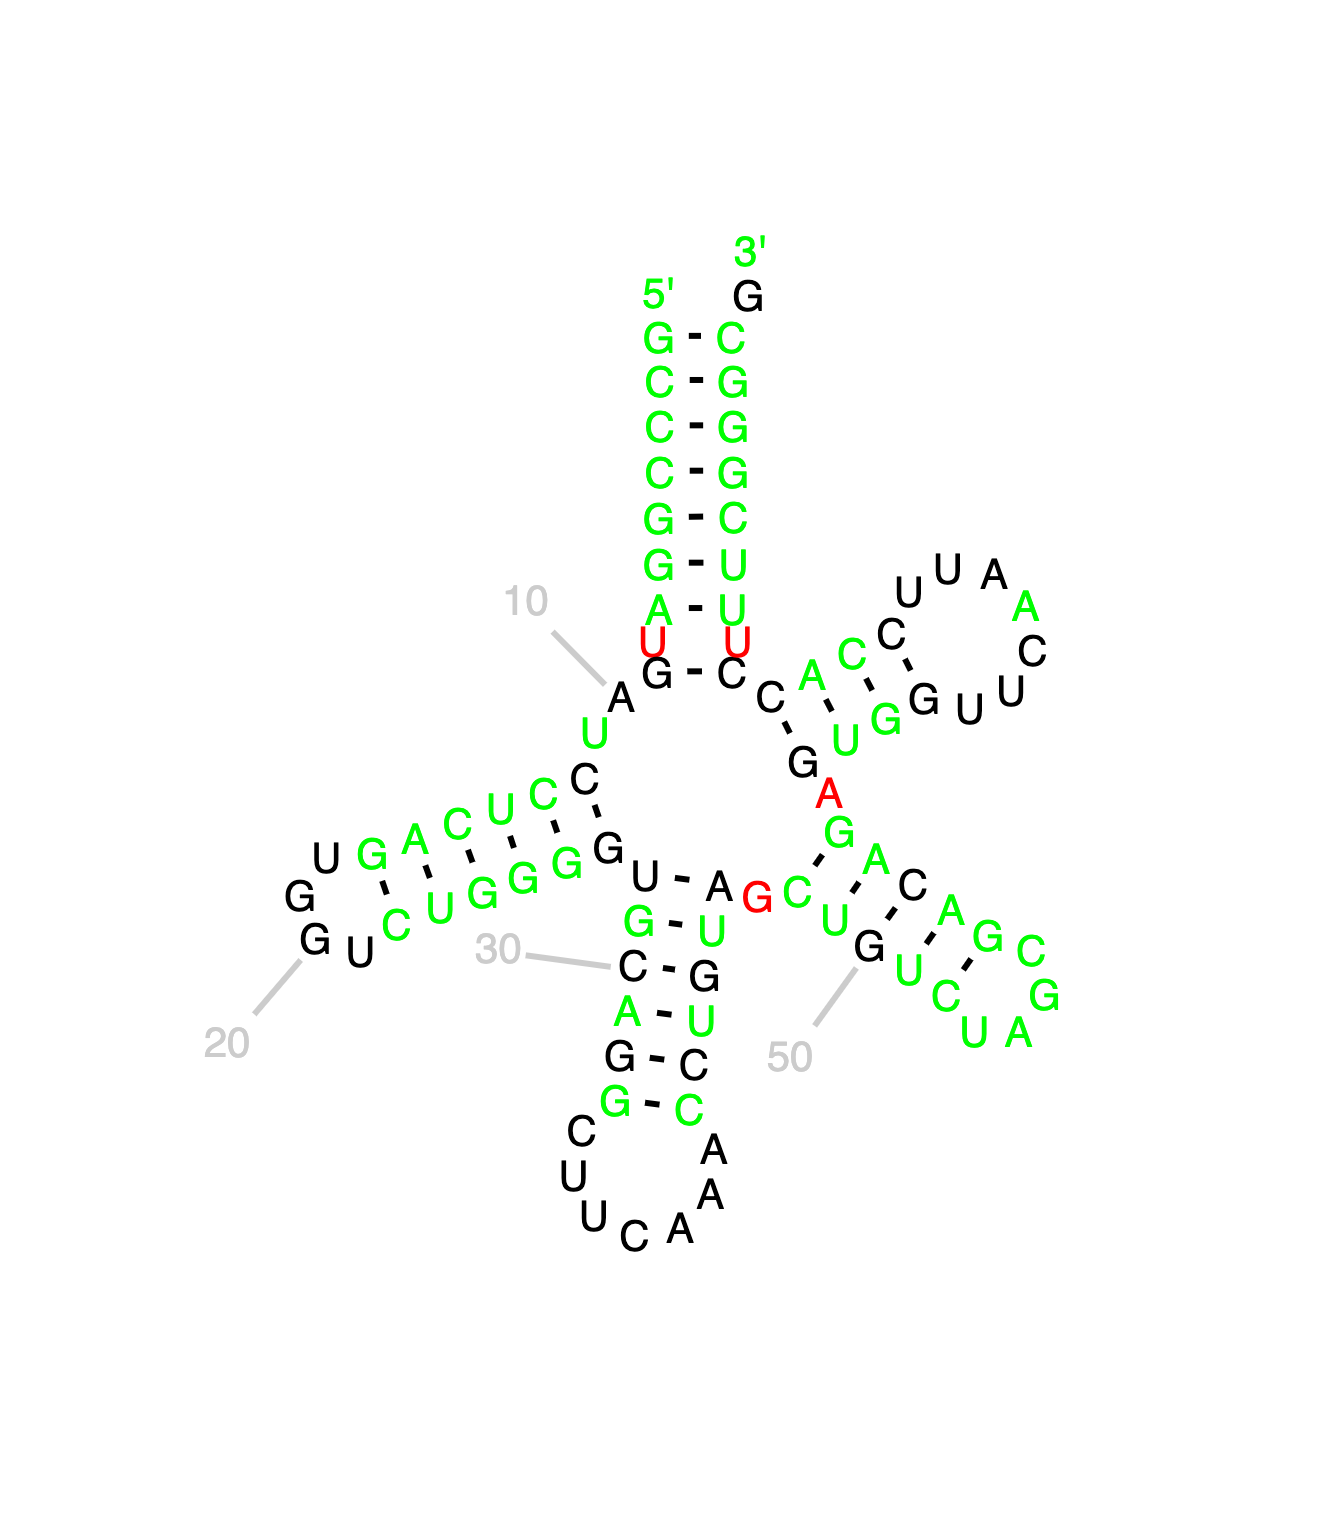
\includegraphics[width=\linewidth]{for_paper1.png}
  \caption{Homo sapiens tRNA-SeC, generated using R2DT secondary structure visualization}
  \label{fig:tRNA}
\end{figure}

As seen in Figure \ref{fig:tRNA},  tRNAs are short sequences which serve as a good benchmark to visualize whether RNA\_LZW is capable of outputting structures that are at all similar to those obtained by tried and true methods of RNA secondary structure discovery. 

Clearly RNA\_Z cannot serve as a replacement for more accurate methods of secondary structure construction; however, the output in Table \ref{tab:tRNA} shows that RNA\_Z is capable of producing somewhat similar structural features to a known dot-bracket structure.  In the case of this tRNA sequence,  RNA\_Z achieves 71\% accuracy when doing a string comparison to the known dot-bracket structure.  This is a quite promising result, especially given RNA\_Z's inability to account for wobble base pairing.

Due to the small size of this sequence, we can see that RNA\_Z's output is clearly different from the known structure, but the hypothesis that RNA\_Z is capable of matching base pairs from any range in the structure is supported by the output generated from this sequence. 

\begin{table}
  \caption{Dot-Bracket Comparison}
  \label{tab:tRNA}
  \begin{tabular}{l}
    \textbf{Sequence}\\
    GCCCGGAUGAUCCUCAGUGGUCUGGGGUGCAGGCUUCA\\
    AACCUGUAGCUGUCUAGCGACAGAGUGGUUCAAUUCCA\\
    CCUUUCGGGCG\\
    \midrule
    \textbf{RNA\_LZW Output}\\
	(((((..(((...))).............((((....((())))...(((((....))))).((((.......)))).)))))))).\\
    \midrule 
    \textbf{Known Dot-Bracket Structure}\\
    (((((((.(..((((((....))))))((((((.......)))))).(((((....))))).((((.......))))).))))))).\\
\end{tabular}
\end{table}


\subsection{Homo sapiens telomerase RNA}

Telomerase is a ribonucleoprotein, meaning that it is a complex structure comprised of non-coding RNA and a protein binding to one another. Telomerase RNA contains a pseudoknot which is integral to telomerase's function [5].  Figure \ref{fig:telomerase} helps visualize how these pseudoknots appear in nature.

Though the length of the sequence (450 nucleotides) means that visual comparison shown in Table \ref{tab:telomerase} is difficult for the reader to assess. When doing a comparison of string similarity, RNA\_Z achieves 51\% accuracy. Once again, assessment of this result must take into account RNA\_Z's inability to detect wobble base pairing. 

\begin{figure}
  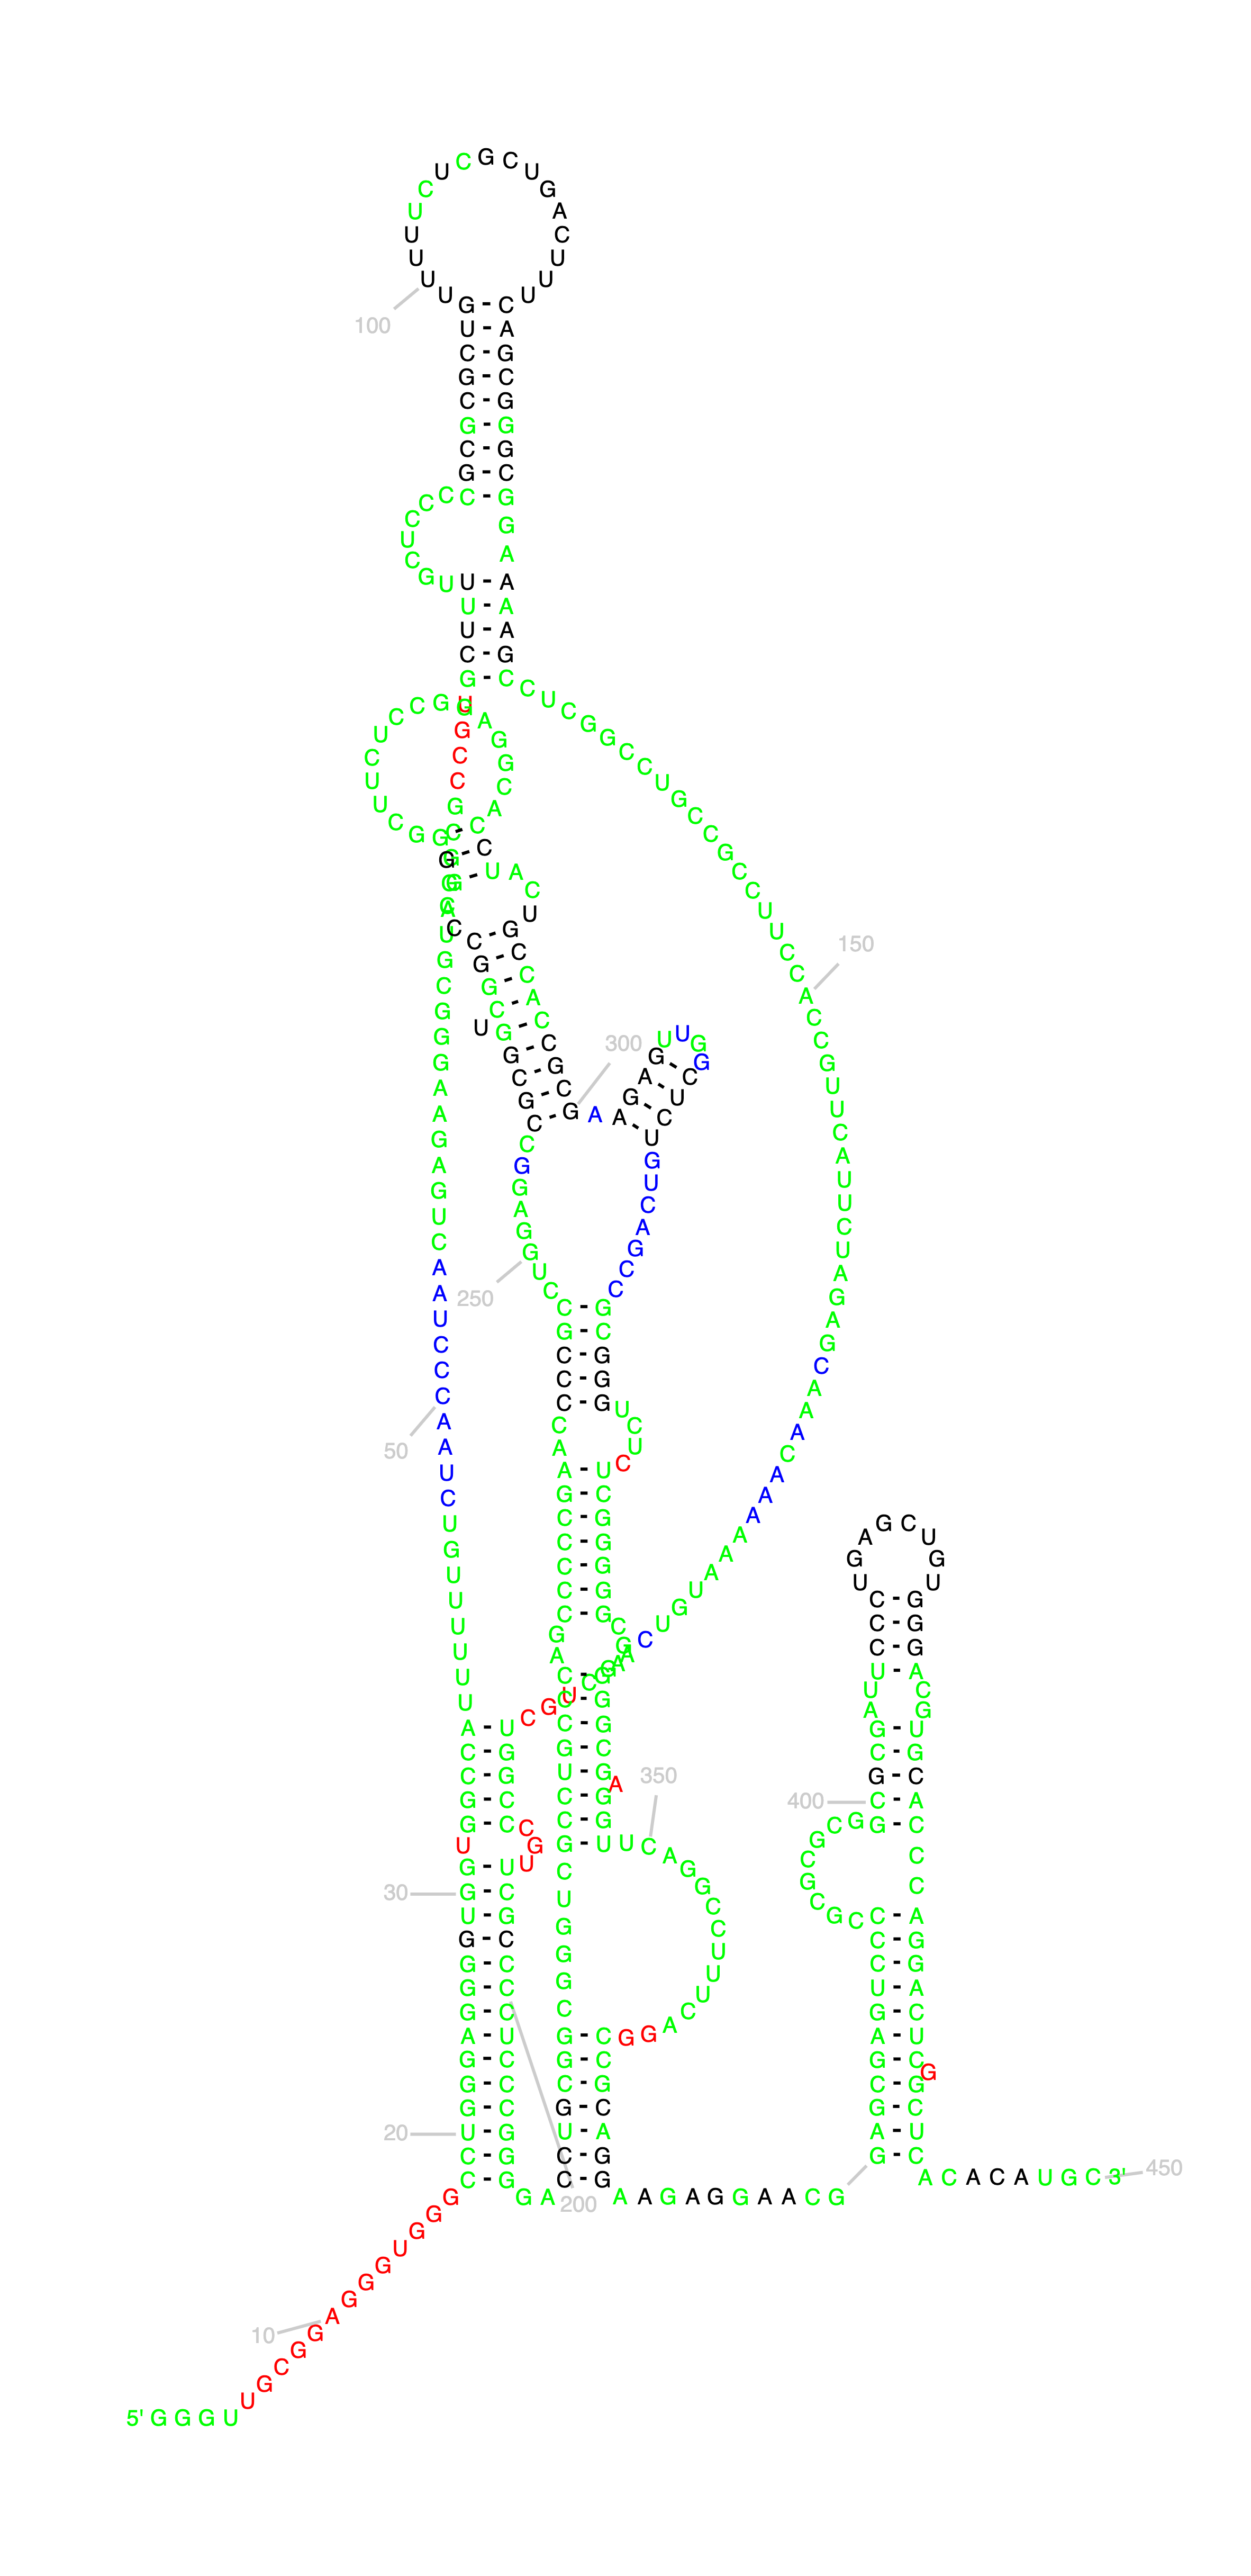
\includegraphics[width=\linewidth]{for_paper.png}
  \caption{Homo sapiens telomerase RNA, generated using R2DT secondary structure visualization}
  \label{fig:telomerase}
\end{figure}


\begin{table}
  \caption{Dot-Bracket Comparison}
  \label{tab:telomerase}
  \begin{tabular}{l}
    \textbf{Sequence}\\
    \midrule
    \textbf{RNA\_LZW Output}\\
    (((((........(((((...(((((((.((((((.(((((((((..))))).....((((((.....(((((.......(((((((.((((((((...\\
    (((((.((((((...))))))....))))).....((((((.)))))................)))))))))))))))..((((.))))..((((((.))\\
    )))))....((((((((((..)))....)))))((((((((.(((((........((((((......))))))))))).......((((...))))))\\
    ....((((....)))).....)))))).....)))))))).......)))).))))))..((((())))))).....))))))..(((((((..))))))))\\
    ........)))))....((((..((()))))))))))))............\\
    \midrule 
    \textbf{Known Dot-Bracket Structure}\\
    .................((((((((((((((.(((((........................................(((((.......(((((((((..............\\
    ...)))))))))..))))).......................................................)))))...))))))))))))))..(((((((......\\
    ((((((((..(((((((..(((((........(((((.((((..(((...............)))...))))))))).((((....)))).......)))))....\\
    )))))))...))))).)))..............)))))))..........(((((((((((........(((((..((((........))))..)))))..)))))))\\
    .))))........
\end{tabular}
\end{table}

\subsection{Homo sapiens RNA, 28S ribosomal N1 (RNA28SN1)}

Ribosomal ribonucleic acid is a primary component of ribosomes which carries out protein synthesis. Thus, rRNA is a prime candidate for testing of larger sequences (5,066 nucleotides). 
In doing a string comparison, RNA\_LZW only achieved 38\% accuracy when analyzed against the known secondary structure.  This low accuracy seems more reasonable once we take into account the lack of wobble base pairing in RNA\_Z's dot bracket structure.  

\begin{figure}
  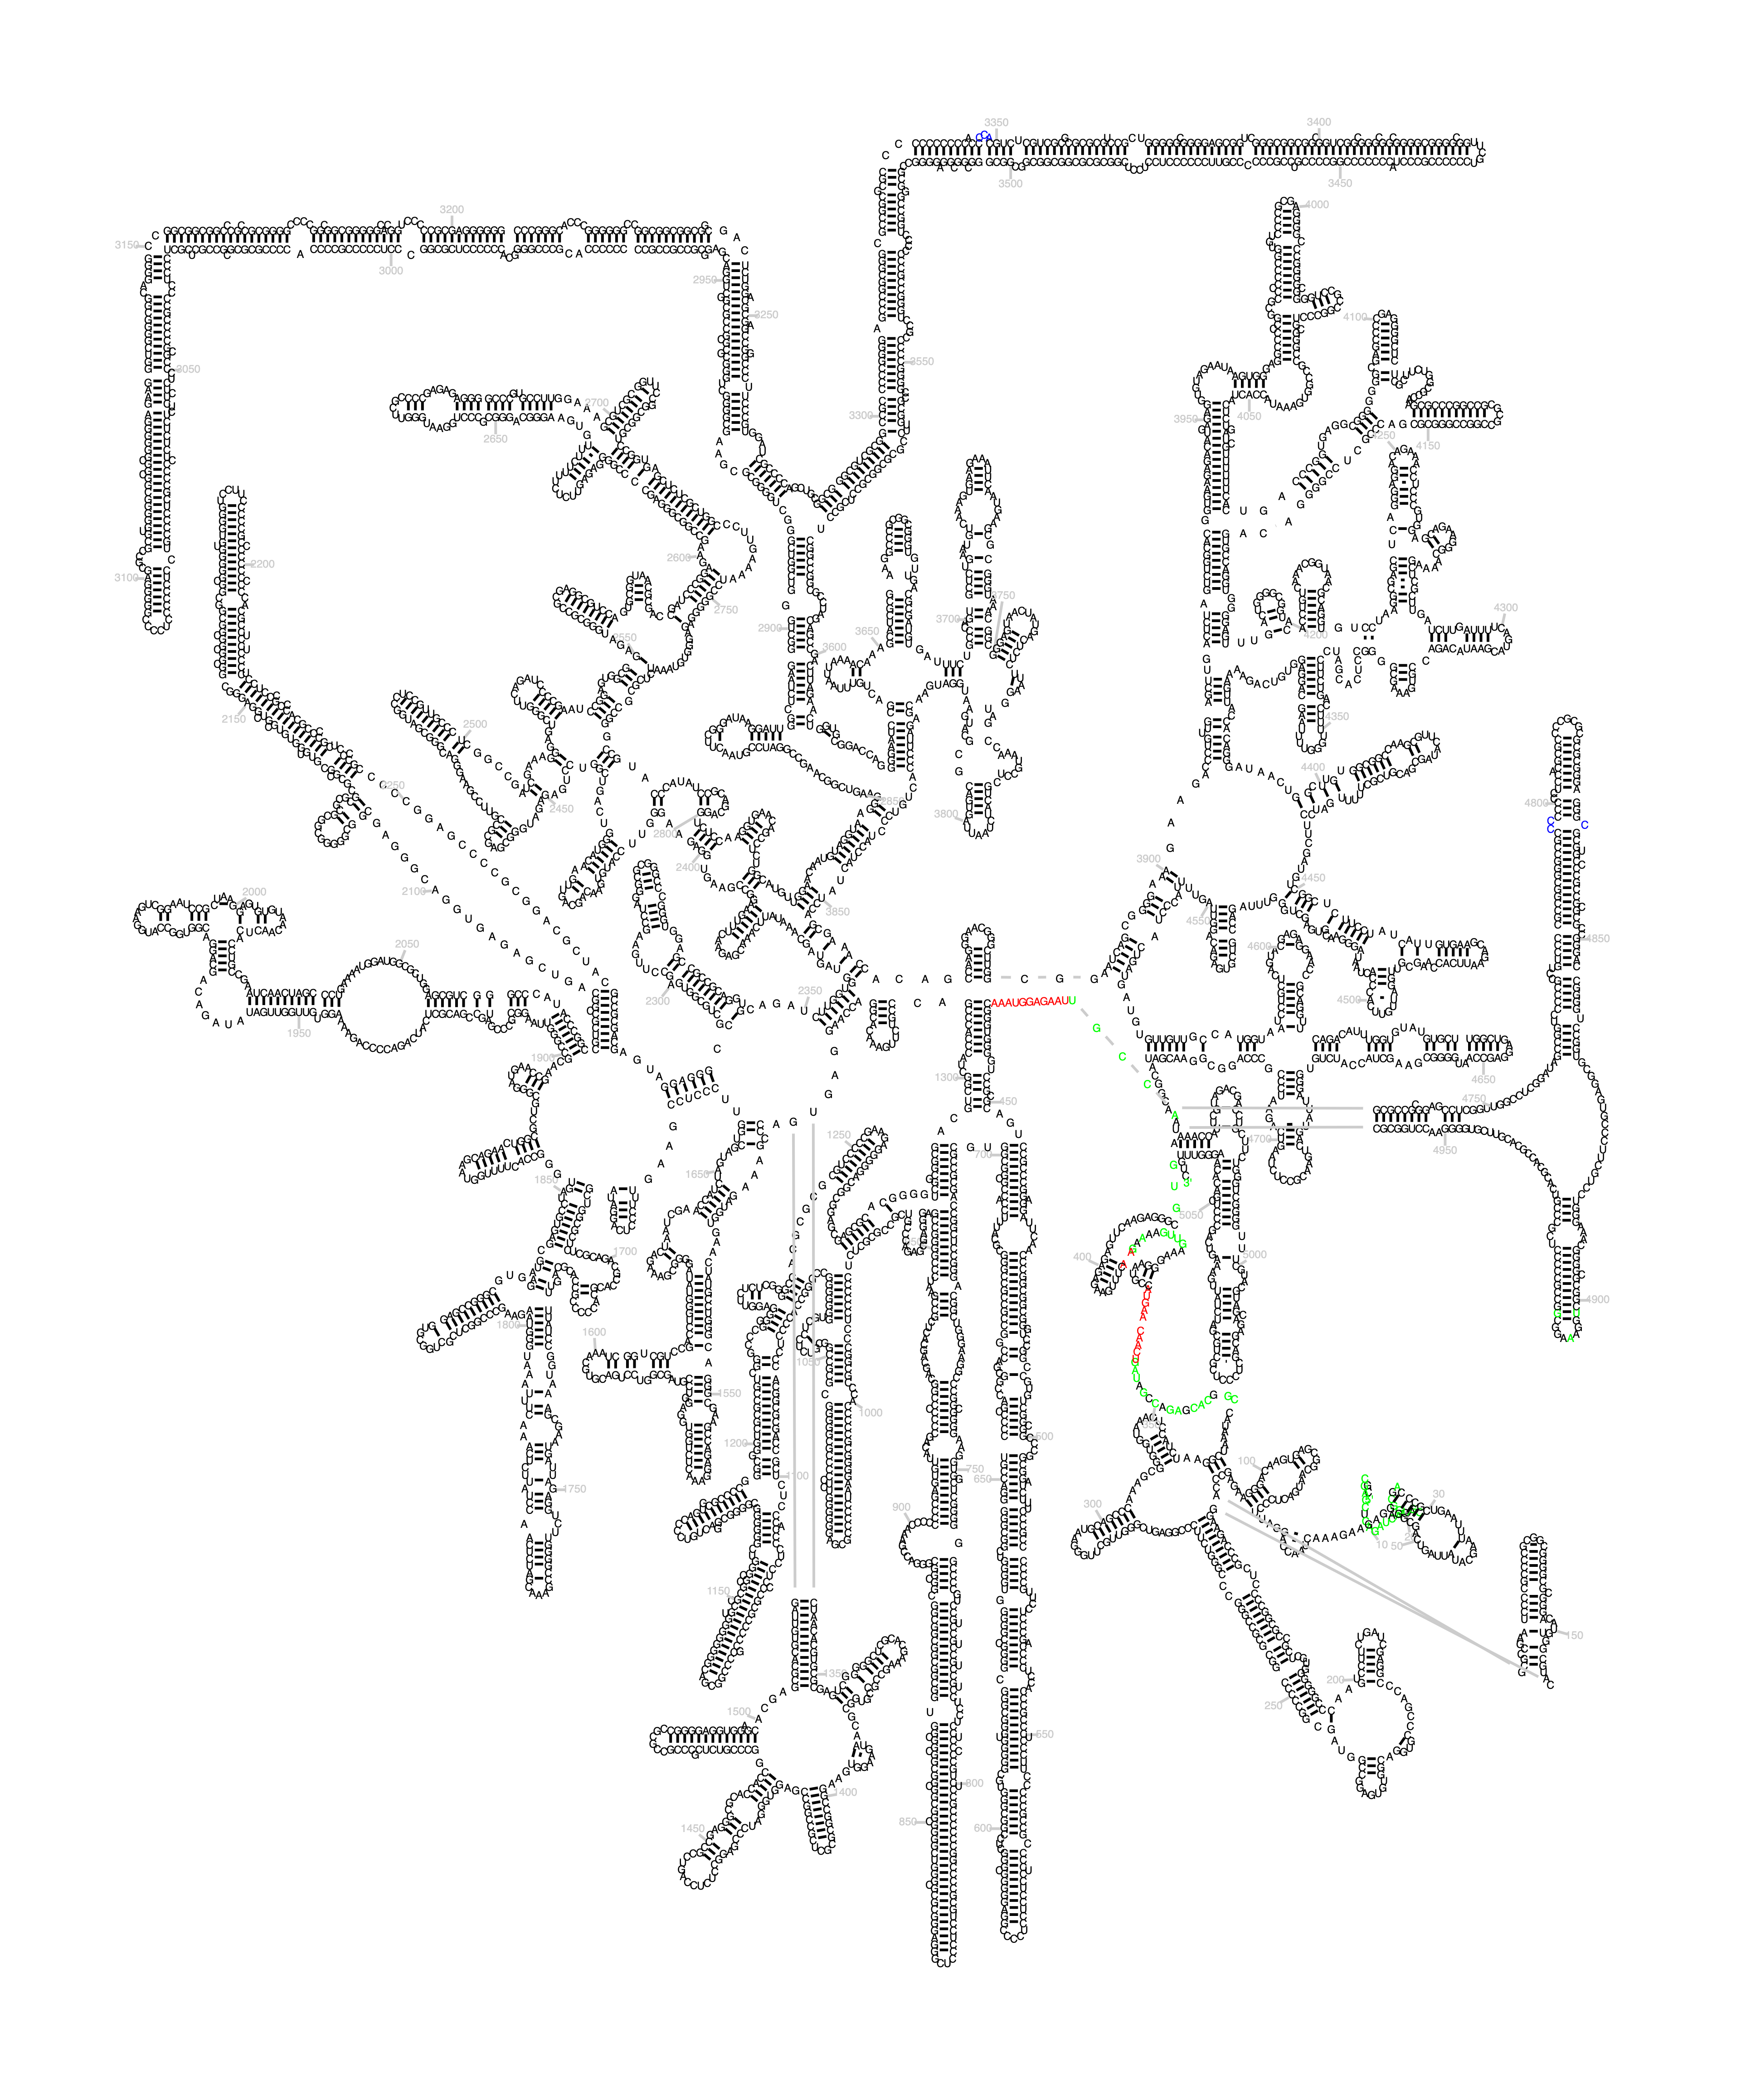
\includegraphics[width=\linewidth]{for_paper2.png}
  \caption{Homo sapiens 28S ribosomal RNA, generated using R2DT secondary structure visualization}
  \label{fig:ribosomal}
\end{figure}


\section{discussion}
%answer the research question, 
%talk to the strengths of what has been found
%talk about limitations
%connect to outside research

Our algorithm shows a remarkable first step towards being able to detect pseudoknots in an efficient manner. Being able to build and parse a dictionary of matches that include pseudoknotted structures in linear time leaves time to improve the metrics by which we parse the dictionary to extract matches, while keeping the entire algorithm efficient. 

The first and most obvious place for improvement is on how we currently choose which dictionary entries make it into the final sequence. Currently we rank first by matching length, and then by distance between them. This is an entirely naive approach that still gave us [[RESULT \%]] accuracy against well known structures. Replacing this naive ordering with a well developed free energy calculation allow the algorithm to select more distant or shorter bonds that end up increasing the stability of the final structure more, and therefore are more likely to be seen in nature.

A second issue is to correct for some artifacts of the LZW algorithm that appear at the start of a sequence. Since the algorithm starts at the first character each loop, and checks against the buffer, the dictionary will never a sequence longer than 2 that starts at the second index, 3 that starts at the 3rd index, and so on. This is a negligable constraint past the first ~50 bases, but could prevent RNA\_LZW from finding good matches on small file sizes. To prevent this an additional step of adding all permutations of the first ~50 bases to the dictionary would fully aleviate this issue. However, since this algorithm is primarily indented to work on large RNA sequences, this is a relatively minor improvement.

The most important next step for this algorithm would be to utilize its strengths of finding likely matches and pseudoknots across arbitrary distances in order to inform more tranditional folding algorithms. By pipelining the output of RNA\_LZW into these more developed algorithms, they can build likely pseudoknotted structures without having to overcome the NP-Complete barrier of having to parse the entire sequence. This is an important step towards being able to efficiently predict the secondary structures of large non-coding RNA sequences. 



\section{conclusion}

The title of your work should use capital letters appropriately -
\url{https://capitalizemytitle.com/} has useful rules for
capitalization. Use the {\verb|title|} command to define the title of
your work. If your work has a subtitle, define it with the
{\verb|subtitle|} command.  Do not insert line breaks in your title.

If your title is lengthy, you must define a short version to be used
in the page headers, to prevent overlapping text. The \verb|title|
command has a ``short title'' parameter:
\begin{verbatim}
  \title[short title]{full title}
\end{verbatim}

\section{Authors and Affiliations}

Each author must be defined separately for accurate metadata
identification. Multiple authors may share one affiliation. Authors'
names should not be abbreviated; use full first names wherever
possible. Include authors' e-mail addresses whenever possible.

Grouping authors' names or e-mail addresses, or providing an ``e-mail
alias,'' as shown below, is not acceptable:
\begin{verbatim}
  \author{Brooke Aster, David Mehldau}
  \email{dave,judy,steve@university.edu}
  \email{firstname.lastname@phillips.org}
\end{verbatim}

The \verb|authornote| and \verb|authornotemark| commands allow a note
to apply to multiple authors --- for example, if the first two authors
of an article contributed equally to the work.

If your author list is lengthy, you must define a shortened version of
the list of authors to be used in the page headers, to prevent
overlapping text. The following command should be placed just after
the last \verb|\author{}| definition:
\begin{verbatim}
  \renewcommand{\shortauthors}{McCartney, et al.}
\end{verbatim}
Omitting this command will force the use of a concatenated list of all
of the authors' names, which may result in overlapping text in the
page headers.

The article template's documentation, available at
\url{https://www.acm.org/publications/proceedings-template}, has a
complete explanation of these commands and tips for their effective
use.

\section{Rights Information}

Authors of any work published by ACM will need to complete a rights
form. Depending on the kind of work, and the rights management choice
made by the author, this may be copyright transfer, permission,
license, or an OA (open access) agreement.

Regardless of the rights management choice, the author will receive a
copy of the completed rights form once it has been submitted. This
form contains \LaTeX\ commands that must be copied into the source
document. When the document source is compiled, these commands and
their parameters add formatted text to several areas of the final
document:
\begin{itemize}
\item the ``ACM Reference Format'' text on the first page.
\item the ``rights management'' text on the first page.
\item the conference information in the page header(s).
\end{itemize}

Rights information is unique to the work; if you are preparing several
works for an event, make sure to use the correct set of commands with
each of the works.

\section{CCS Concepts and User-Defined Keywords}

Two elements of the ``acmart'' document class provide powerful
taxonomic tools for you to help readers find your work in an online
search.

The ACM Computing Classification System ---
\url{https://www.acm.org/publications/class-2012} --- is a set of
classifiers and concepts that describe the computing
discipline. Authors can select entries from this classification
system, via \url{https://dl.acm.org/ccs/ccs.cfm}, and generate the
commands to be included in the \LaTeX\ source.

User-defined keywords are a comma-separated list of words and phrases
of the authors' choosing, providing a more flexible way of describing
the research being presented.

CCS concepts and user-defined keywords are required for all short- and
full-length articles, and optional for two-page abstracts.

\section{Sectioning Commands}

Your work should use standard \LaTeX\ sectioning commands:
\verb|section|, \verb|subsection|, \verb|subsubsection|, and
\verb|paragraph|. They should be numbered; do not remove the numbering
from the commands.

Simulating a sectioning command by setting the first word or words of
a paragraph in boldface or italicized text is {\bfseries not allowed.}

\section{Tables}

The ``\verb|acmart|'' document class includes the ``\verb|booktabs|''
package --- \url{https://ctan.org/pkg/booktabs} --- for preparing
high-quality tables.

Table captions are placed {\itshape above} the table.

Because tables cannot be split across pages, the best placement for
them is typically the top of the page nearest their initial cite.  To
ensure this proper ``floating'' placement of tables, use the
environment \textbf{table} to enclose the table's contents and the
table caption.  The contents of the table itself must go in the
\textbf{tabular} environment, to be aligned properly in rows and
columns, with the desired horizontal and vertical rules.  Again,
detailed instructions on \textbf{tabular} material are found in the
\textit{\LaTeX\ User's Guide}.

Immediately following this sentence is the point at which
Table~\ref{tab:freq} is included in the input file; compare the
placement of the table here with the table in the printed output of
this document.

\begin{table}
  \caption{Frequency of Special Characters}
  \label{tab:freq}
  \begin{tabular}{ccl}
    \toprule
    Non-English or Math&Frequency&Comments\\
    \midrule
    \O & 1 in 1,000& For Swedish names\\
    $\pi$ & 1 in 5& Common in math\\
    \$ & 4 in 5 & Used in business\\
    $\Psi^2_1$ & 1 in 40,000& Unexplained usage\\
  \bottomrule
\end{tabular}
\end{table}

To set a wider table, which takes up the whole width of the page's
live area, use the environment \textbf{table*} to enclose the table's
contents and the table caption.  As with a single-column table, this
wide table will ``float'' to a location deemed more
desirable. Immediately following this sentence is the point at which
Table~\ref{tab:commands} is included in the input file; again, it is
instructive to compare the placement of the table here with the table
in the printed output of this document.

\begin{table*}
  \caption{Some Typical Commands}
  \label{tab:commands}
  \begin{tabular}{ccl}
    \toprule
    Command &A Number & Comments\\
    \midrule
    \texttt{{\char'134}author} & 100& Author \\
    \texttt{{\char'134}table}& 300 & For tables\\
    \texttt{{\char'134}table*}& 400& For wider tables\\
    \bottomrule
  \end{tabular}
\end{table*}

\section{Math Equations}
You may want to display math equations in three distinct styles:
inline, numbered or non-numbered display.  Each of the three are
discussed in the next sections.

\subsection{Inline (In-text) Equations}
A formula that appears in the running text is called an inline or
in-text formula.  It is produced by the \textbf{math} environment,
which can be invoked with the usual
\texttt{{\char'134}begin\,\ldots{\char'134}end} construction or with
the short form \texttt{\$\,\ldots\$}. You can use any of the symbols
and structures, from $\alpha$ to $\omega$, available in
\LaTeX~\cite{Lamport:LaTeX}; this section will simply show a few
examples of in-text equations in context. Notice how this equation:
\begin{math}
  \lim_{n\rightarrow \infty}x=0
\end{math},
set here in in-line math style, looks slightly different when
set in display style.  (See next section).

\subsection{Display Equations}
A numbered display equation---one set off by vertical space from the
text and centered horizontally---is produced by the \textbf{equation}
environment. An unnumbered display equation is produced by the
\textbf{displaymath} environment.

Again, in either environment, you can use any of the symbols and
structures available in \LaTeX\@; this section will just give a couple
of examples of display equations in context.  First, consider the
equation, shown as an inline equation above:
\begin{equation}
  \lim_{n\rightarrow \infty}x=0
\end{equation}
Notice how it is formatted somewhat differently in
the \textbf{displaymath}
environment.  Now, we'll enter an unnumbered equation:
\begin{displaymath}
  \sum_{i=0}^{\infty} x + 1
\end{displaymath}
and follow it with another numbered equation:
\begin{equation}
  \sum_{i=0}^{\infty}x_i=\int_{0}^{\pi+2} f
\end{equation}
just to demonstrate \LaTeX's able handling of numbering.

\section{Citations and Bibliographies}

The use of or the preparation and formatting of one's
references is strongly recommended. Authors' names should be complete
--- use full first names (``Donald E. Knuth'') not initials
(``D. E. Knuth'') --- and the salient identifying features of a
reference should be included: title, year, volume, number, pages,
article DOI, etc.

The bibliography is included in your source document with these two
commands, placed just before the \verb|\end{document}| command:
\begin{verbatim}
  \bibliographystyle{ACM-Reference-Format}
  \bibliography{bibfile}
\end{verbatim}
where ``\verb|bibfile|'' is the name, without the ``\verb|.bib|''
suffix, of th.

Citations and references are numbered by default. A small number of
ACM publications have citations and references formatted in the
``author year'' style; for these exceptions, please include this
command in the {\bfseries preamble} (before
``\verb|\begin{document}|'') of your \LaTeX\ source:
\begin{verbatim}
  \citestyle{acmauthoryear}
\end{verbatim}


\section{Acknowledgments}

Identification of funding sources and other support, and thanks to
individuals and groups that assisted in the research and the
preparation of the work should be included in an acknowledgment
section, which is placed just before the reference section in your
document.

This section has a special environment:
\begin{verbatim}
  \begin{acks}
  ...
  \end{acks}
\end{verbatim}
so that the information contained therein can be more easily collected
during the article metadata extraction phase, and to ensure
consistency in the spelling of the section heading.

Authors should not prepare this section as a numbered or unnumbered {\verb|\section|}; please use the ``{\verb|acks|}'' environment.

\section{Appendices}

If your work needs an appendix, add it before the
``\verb|\end{document}|'' command at the conclusion of your source
document.

Start the appendix with the ``\verb|appendix|'' command:
\begin{verbatim}
  \appendix
\end{verbatim}
and note that in the appendix, sections are lettered, not
numbered. This document has two appendices, demonstrating the section
and subsection identification method.

\section{SIGCHI Extended Abstracts}

The ``\verb|sigchi-a|'' template style (available only in \LaTeX\ and
not in Word) produces a landscape-orientation formatted article, with
a wide left margin. Three environments are available for use with the
``\verb|sigchi-a|'' template style, and produce formatted output in
the margin:
\begin{itemize}
\item {\verb|sidebar|}:  Place formatted text in the margin.
\item {\verb|marginfigure|}: Place a figure in the margin.
\item {\verb|margintable|}: Place a table in the margin.
\end{itemize}

%%
%% The acknowledgments section is defined using the "acks" environment
%% (and NOT an unnumbered section). This ensures the proper
%% identification of the section in the article metadata, and the
%% consistent spelling of the heading.
\begin{acks}
To Robert, for the bagels and explaining CMYK and color spaces.
\end{acks}

%%
%% The next two lines define the bibliography style to be used, and
%% the bibliography file.
\bibliographystyle{ACM-Reference-Format}
\bibliography{sample-base}

%%
%% If your work has an appendix, this is the place to put it.
\appendix

\section{Research Methods}

\subsection{Part One}

\section{bibliography}
\begin{thebibliography}{10}
	\bibitem{RNAZ2} A. R. Gruber S. Findeiß, S. Washietl, I. L. Hofacker, and P. F. Stadler, “RNAZ 2.0: Improved Noncoding RNA Detection,” Pacific Symposium on Biocomputing, pp. 69–79, 2010. 
	\bibitem{Fast} S. Washietl, I. L. Hofacker, and P. F. Stadler, “Fast and Reliable Prediction of Noncoding RNAs,” Proceedings of the National Academy of Sciences, vol. 102 (7), pp. 2454–2459, 2005.  
	\bibitem{compres} T. A. Welch, "A Technique for High-Performance Data Compression," in Computer, vol. 17, no. 6, pp. 8-19, June 1984, doi: 10.1109/MC.1984.1659158.
	\bibitem{RNAFold} I. L. Hofacker, S. Bonhoeffer, P. F. Stadler, R. Lorenz, and W. Fontana, “RNAfold manual page for RNAfold 2.4.16,” Theoretical Biochemistry Group. [Online]. Available: \url{https://www.tbi.univie.ac.at/RNA/RNAfold.1.html#heading7}. [Accessed: 21-Feb-2021]. 
	\bibitem{ncbi} https://www.ncbi.nlm.nih.gov/pmc/articles/PMC21964/
	\bibitem{NP} Lyngsø, Rune and Pedersen, Christian. (2000). RNA Pseudoknot Prediction in Energy-Based Models. Journal of computational biology : a journal of computational molecular cell biology. 7. 409-27. 10.1089/106652700750050862. 
\end{thebibliography}

\end{document}
\endinput
%%
%% End of file `sample-sigconf.tex'.
